\section{Databehandling}
\subsection{Afbildning med én samlelinse}
<<<<<<< HEAD
<<<<<<< HEAD
I dette forsøg, ændres positionen for linsen hvorefter positionen af skærmens position ændres, så billedet igen står skarpt. Der ønskes altså at undersøge sammenhængen mellem \cref{eq:formel}.
Vores resultater kan ses på
\begin{table}[H]
    \begin{tabular}{c|c|c|c|c|c|c|c|c|c|c}
        58 &  64 &  59 &  57 &  57 &  57  & 59  & 61  & ...
    \end{tabular}
=======
I dette forsøg, ændres positionen for linsen hvorefter positionen af skærmens position ændres, så billedet igen står skarpt. Der ønskes altså at undersøge sammenhængen mellem \cref{eq:formel}. Afstanden skiftes mens $s$ og $s'$ bestemmes så billedet står skarpt igen på skærmen.
Vores resultater kan ses på \cref{fig:res1}.
\begin{figure}[H]
    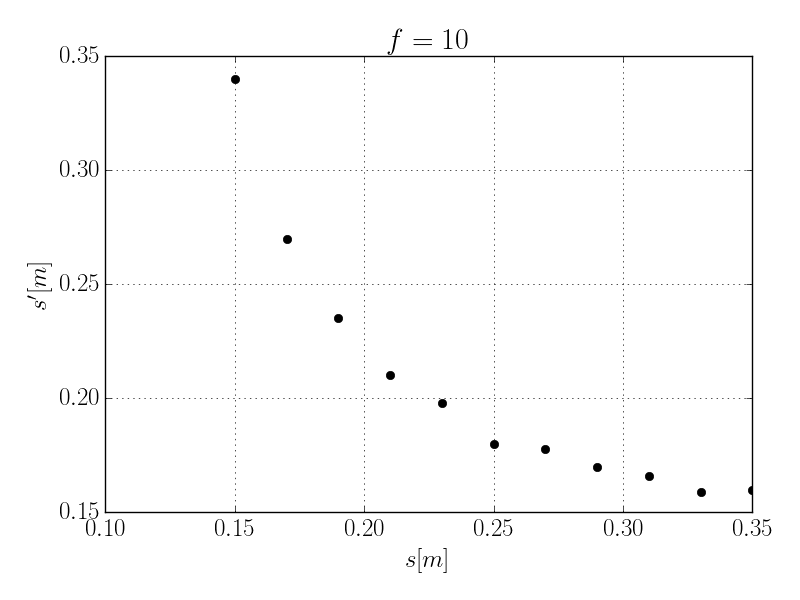
\includegraphics[width=\linewidth]{res1.png}
>>>>>>> b1ed865b8b254c8973ed35589aa1914324b36f20
    \caption{}
=======
I dette forsøg, ændres positionen for linsen hvorefter positionen af skærmens position ændres, så billedet igen står skarpt. Der ønskes altså at undersøge sammenhængen mellem \cref{eq:fokalvokal}. Afstanden skiftes mens $s$ og $s'$ bestemmes så billedet står skarpt igen på skærmen.
Vores resultater kan ses på \cref{fig:res1}.
\begin{figure}[H]
    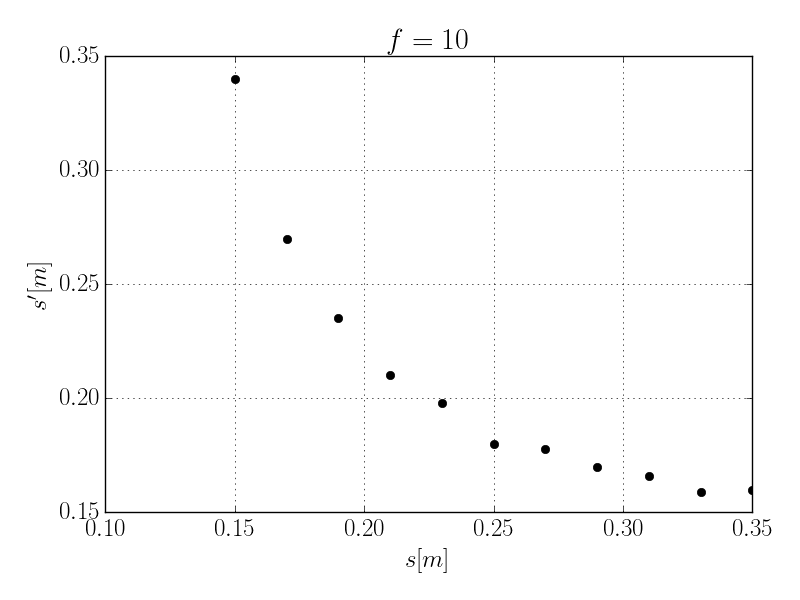
\includegraphics[width=\linewidth]{res1.png}
    \caption{Resultater af forsøg 1}
>>>>>>> 7c6d3c162910dc2625ce29bbf44eb448ce9d78ed
    \label{fig:res1}
\end{figure}


\begin{figure}[H]
    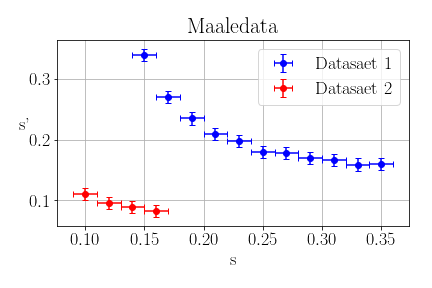
\includegraphics[width=\linewidth]{usikkerhed.png}
    \caption{}
    \label{fig:usikkerhed}
\end{figure}

\begin{figure}[H]
    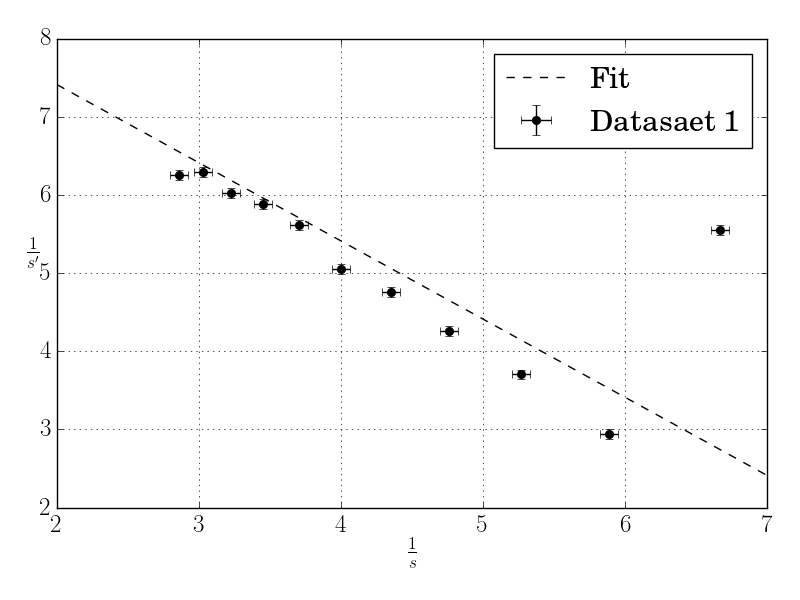
\includegraphics[width=\linewidth]{1.png}
    \caption{}
    \label{fig:1}
\end{figure}

\begin{figure}[H]
    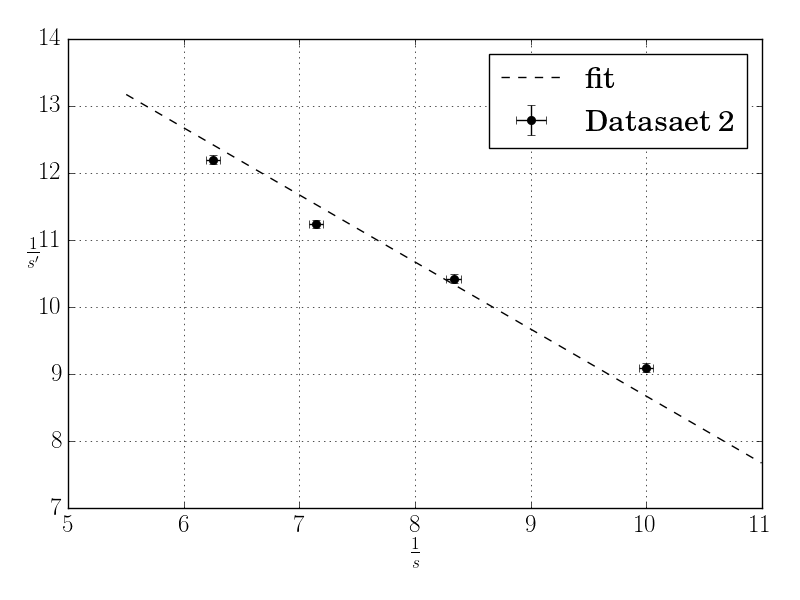
\includegraphics[width=\linewidth]{2.png}
    \caption{}
    \label{fig:2}
\end{figure}

\begin{figure}[H]
    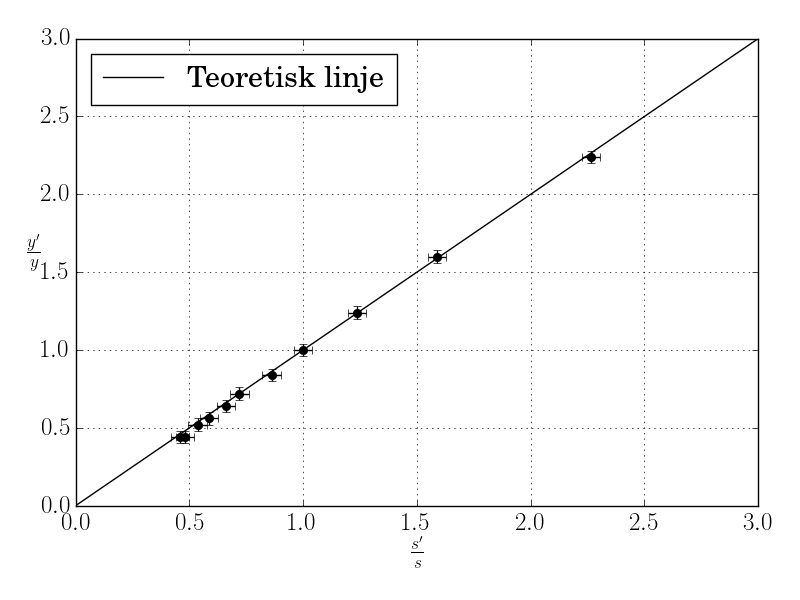
\includegraphics[width=\linewidth]{3.png}
    \caption{}
    \label{fig:3}
\end{figure}
